%!TEX root = main.tex
%%% Review Material and Basics of Equations
\part{}
\renewcommand{\thesection}{\Alph{section}}
\setcounter{section}{17}
% \section*{Review Material}\addcontentsline{toc}{section}{Review Material}
\section{Review Material}

\subsection{Rational Exponents \& Radicals}

\begin{fact}
For any real number $\mathbf{a}$ the following holds:
\ifprintanswers
\begin{LargeEq}
a^{\frac{m}{n}}=\sqrt[n]{a^m}
\end{LargeEq}
\else
\begin{LargeEq}
a^{\frac{m}{n}}=\sqrt[\rule{5pt}{0.5pt}]{a^{\rule{5pt}{0.5pt}}}
\end{LargeEq}
\fi
\end{fact}
\begin{exercise}
Rewrite $3^{\frac{2}{3}}$ as a radical.
\end{exercise}
\begin{solution}[2in]
\[
3^{\frac{2}{3}}=\sqrt[3]{3^2}=\sqrt[3]{9}
\]
\answer{$\sqrt[3]{9}$}
\end{solution}
\vspace{.5em}
\begin{exercise}
Rewrite $\sqrt[5]{16}$ as a rational exponent.
\end{exercise}
\begin{solution}[2in]
We have two options. The first is
\begin{align*}
\sqrt[5]{16}&=16^{\frac{1}{5}}\\
&=\left(4^2\right)^{\frac{1}{5}}\\
&=4^{\frac{2}{5}}\\
&=\left(2^2\right)^{\frac{2}{5}}\\
&=2^{\frac{4}{5}}
\end{align*}
Otherwise, we could work inside the radical first
\begin{align*}
\sqrt[5]{16}&=\sqrt[5]{2^4}\\
&=2^{\frac{4}{5}}
\end{align*}
\answer{$2^{\frac{4}{5}}$}
\end{solution}
\vspace{0.5em}

\newpage
\subsubsection{Simplifying Radicals}

We have two techniques on how to simplify radicals. One is called the \emph{factor tree method},
and the other involves looking at powers of primes.

\begin{exercise}[Factor Tree Method]
Simplify $\sqrt{72}$.
\end{exercise}
\begin{solution}[2in]
We begin by drawing the following tree-like diagram of factors of 72.
\begin{center}
\begin{tikzpicture}
\node(Root)                                             {$\sqrt{72}$};
\node(11)   [below left = 0.5cm and 0.5cm of Root]      {$2$};
\node(12)   [below right = 0.5cm and 0.5cm of Root]     {$36$};
\node(21)   [below left = 0.5cm and 0.5cm of 12]        {$6$};
\node(22)   [below right = 0.5cm and 0.5cm of 12]       {$6$};
\node(31)   [below left = 0.5cm and 0.5cm of 21]        {$2$};
\node(32)   [below right = 0.5cm and 0.3cm of 21]       {$3$};
\node(33)   [below left = 0.5cm and 0.3cm of 22]        {$3$};
\node(34)   [below right = 0.5cm and 0.5cm of 22]       {$2$};

\foreach \x in {1,2} {
\draw[black] (Root)--(1\x);
\draw[black] (12)--(2\x);
\draw[black] (21)--(3\x);
}
\foreach \x in {3,4} {
\draw[black] (22)--(3\x);
}
\end{tikzpicture}
\end{center}
We now look at the end of the branches which in this case are ``2,2,3,3,2''
going from left to right.

Since this is a \textbf{square root} we want to look for \textbf{pairs} of numbers
(cube root=triples, fourth root=groups of four, etc.). There is one pair of 2's and
a pair of 3's, and one 2 left over. For each pair of a number, we write one of it
outside the radical, and we multiply all the remaining numbers back together under
the radical. So for this problem we have
\[
2\cdot3\sqrt{2}=6\sqrt{2}
\]
\answer{$6\sqrt{2}$}.
\end{solution}
\vspace{0.5em}

\begin{exercise}[Powers of Primes Method]
Simplify $\sqrt{72}$.
\end{exercise}
\begin{solution}[1.5in]
In this method we write $72$ in it's \emph{prime-factorization}, that is we
write it as a product of powers of primes.
\[
72=8\cdot9=2^3\cdot3^2.
\]
Now that we know that $72=2^3\cdot3^2$, we will use that the square root is
the same as the $\frac{1}{2}$-power.
\begin{align*}
\sqrt{72}&=\sqrt{2^3\cdot3^2}\\
&=\left(2^3\cdot3^2\right)^{\frac{1}{2}}\\
&=2^{\frac{3}{2}}\cdot3^{\frac{2}{2}}\\
&=2^{1\frac{1}{2}}\cdot3^{1}\\
&=2^1\cdot3^1\cdot2^{\frac{1}{2}}\\
&=2\cdot3\sqrt{2}\\
&=6\sqrt{2}
\end{align*}
\answer{$6\sqrt{2}$}
\end{solution}
\vspace{0.5em}
\begin{exercise}
Simplify $\sqrt[3]{500}$.
\end{exercise}
\begin{solution}[3in]

\end{solution}

\subsection{Polynomials}
\subsubsection{Basics}
\begin{definition}\label{def: polynomial}
Let $n$ be a positive integer (not a fraction), and $a_0,a_1,a_2,\ldots,a_{n-1},a_n$ be real
numbers with $a_n\neq0$. The following is called a \emph{polynomial}:
\[
a_nx^n+a_{n-1}x^{n-1}+\cdots+a_1x+a_0.
\]
\begin{itemize}
    \item We call $a_0,a_1,\ldots,a_n$ the \ifprintanswers\emph{coefficients}\else\rule{60pt}{.5pt}\fi,
    \item $a_n$ is specifically called the \ifprintanswers\emph{leading coefficient}\else\rule{60pt}{.5pt}\fi,
    \item $a_nx^n$ is called the \ifprintanswers\emph{leading term}\else\rule{60pt}{.5pt}\fi,
    \item $a_0$ is called the \ifprintanswers\emph{constant term}\else\rule{60pt}{.5pt}\fi,
    \item and $n$ is the \ifprintanswers\emph{leading coefficient}~\else\rule{60pt}{.5pt}~\fi of the polynomial.
\end{itemize}
\end{definition}
\begin{center}
Names based on the number of terms
\vspace{0.3em}\\
\begin{tabular}{|c|c|}
\hline
\# of Terms & Name \\
\hline
$1$ & \ifprintanswers monomial\else\phantom{monomial}\fi\\
\hline
$2$ & \ifprintanswers binomial\else\phantom{binomial}\fi\\
\hline
$3$ & \ifprintanswers trinomial\else\phantom{trinomial}\fi\\
\hline
$4$ or more & \ifprintanswers polynomial\else\phantom{polynomial}\fi\\
\hline
\end{tabular}
\end{center}
\begin{center}
Names based on the degree
\vspace{0.3em}\\
\begin{tabular}{|c|c|}
\hline
Degree & Name \\
\hline
$0$th & \ifprintanswers constant\else\phantom{==constant==}\fi\\
\hline
$1$st & \ifprintanswers linear\else\phantom{==linear==}\fi\\
\hline
$2$nd & \ifprintanswers quadratic\else\phantom{==quadratic==}\fi\\
\hline
$3$rd & \ifprintanswers cubic\else\phantom{==cubic==}\fi\\
\hline
$4$th & \ifprintanswers quartic\else\phantom{==quartic==}\fi\\
\hline
$5$th & \ifprintanswers quintic\else\phantom{==quintic==}\fi\\
\hline
\end{tabular}
\end{center}

\begin{exercise}
What special name(s) would the following polynomials have?
\begin{itemize}
    \item $3x^2+x-1$\quad Name: \ifprintanswers quadratic or trinomial \else \rule{60pt}{0.5pt}\fi
    \item $7+-4x^3$\quad Name: \ifprintanswers cubic or binomial \else \rule{60pt}{0.5pt}\fi
\end{itemize}
\end{exercise}

\newpage

\subsubsection{Adding and Subtracting}
When adding or subtracting polynomials it boils down to combining the coefficients of \emph{like-terms}
that is terms that have the same power of $x$.
\begin{exercise}
Add the following two polynomials together:
\[
(3x^2+x+1)+(3-6x-2x^2)
\]
\end{exercise}
\begin{solution}[1.5in]
Each term in the first polynomial has a like term in the second. This does not
always happen, but since it does here we will have to combine the 3 pairs.
\[
(3x^2+x+1)+(3-6x-2x^2)
\]
\[
(3x^2+-2x^2)+(x+-6x)+(1+3)
\]
\[
(3x^2-2x^2)+(x-6x)+(1+3)
\]
\[
x^2-5x+4
\]
\answer{$x^2-5x+4$}
\end{solution}
\vspace{0.5em}

\begin{exercise}
Compute the following subtraction of polynomials:
\[
(1-x-5x^2)-(-3x^2+4x-3)
\]
\end{exercise}
\begin{solution}[1.5in]
As we saw that addition is relatively straight forward, are goal will be to
rewrite any subtraction problem as addition.
\[
(1-x-5x^2)-(-3x^2+4x-3)
\]
\[
(1-x-5x^2)+-1(-3x^2+4x-3)
\]
\[
(1-x-5x^2)+(3x^2-4x+3)
\]
\[
(-5x^2+3x^2)+(-x+-4x)+(1+3)
\]
\[
-2x^2-5x+4
\]
\answer{$-2x^2-5x+4$}
\end{solution}
\vspace{0.5em}

\subsubsection{Multiplying}

The basic premise of multiplication of polynomials is multiplying coefficients and
adding powers.
\[
(Ax^n)(Bx^m)=ABx^{n+m}
\]

\begin{exercise}
Compute the following multiplication:
\[
(3x)(2x)
\]
\end{exercise}
\begin{solution}[2in]
Recall that if there is no power written that it to the power of $1$, so
\[
(3x)(2x)=(3x^1)(2x^1)=6x^2
\]
\answer{$6x^2$}
\end{solution}
\vspace{0.5em}

\begin{definition}
When multiplying two binomials we use an acronym to help remember which terms
to multiply together, which is \textbf{F.O.I.L.}.
\begin{center}
\ifprintanswers
\textbf{F}\underline{irst}\quad\textbf{O}\underline{utside}
\quad\textbf{I}\underline{nside}\quad\textbf{L}\underline{ast}
\else
\textbf{F}\underline{\phantom{========}}\quad\textbf{O}\underline{\phantom{========}}
\quad\textbf{I}\underline{\phantom{========}}\quad\textbf{L}\underline{\phantom{========}}
\fi
\end{center}
\end{definition}
\vspace{0.5em}

\begin{exercise}
Multiply the following binomials:
\[
(2x+7)(3x-4)
\]
\end{exercise}
\begin{solution}[2in]
First a visualization of F.O.I.L.
\begin{center}
\begin{tikzpicture}
\node(AP1)                       {$($};
\node(A1)   [right=.01cm of AP1]  {$2x$};
\node(AP)   [right=.01cm of A1]   {$+$};
\node(A2)   [right=.01cm of AP]   {$7$};
\node(AP2)  [right=.01cm of A2]   {$)$};
\node(BP1)  [right=.01cm of AP2]  {$($};
\node(B1)   [right=.01cm of BP1]  {$3x$};
\node(BP)   [right=.01cm of B1]   {$-$};
\node(B2)   [right=.01cm of BP]   {$4$};
\node(BP2)  [right=.01cm of B2]   {$)$};
\foreach \x in {1,2}
\foreach \y in {1,2} {
\draw[blue] (A\x) to[out=40,in=140] (B\y);
}
\end{tikzpicture}    
\end{center}
For each line we have a multiplication pair. This lead us to the following
\begin{align*}
(2x+7)(3x-4)&=(2x)(3x)+(2x)(-4)+(7)(3x)+(7)(-4)\\
&=6x^2-8x+21x-28\\
&=6x^2{\color{blue}-8x+21x}-28\\
&=6x^2+13x-28
\end{align*}
\answer{$6x^2+13x-28$}
\end{solution}
\vspace{0.5em}

\begin{exercise}
Simplify the following:
\[
(5x+2)^2
\]
\end{exercise}
\begin{solution}[2in]
Recall that $a^2=a\cdot a$, so
\begin{align*}
(5x+2)^2&=(5x+2)(5x+2)\\
&=(5x)(5x)+(5x)(2)+(2)(5x)+(2)(2)\\
&=25x^2+10x+10x+4\\
&=25x^2+20x+4
\end{align*}
\answer{$25x^2+20x+4$}
\begin{note}
We call this type of polynomial a \emph{perfect square trinomial}.
\end{note}
\end{solution}
\vspace{0.5em}
\begin{exercise}
Multiply the following binomials:
\[
(3x+1)(3x-1)
\]
\end{exercise}
\begin{solution}[2in]
Again we will use the F.O.I.L. method:
\begin{align*}
(3x+1)(3x-1)&=(3x)(3x)+(3x)(-1)+(1)(3x)+(1)(-1)\\
&=9x^2-3x+3x-1\\
&=9x^2-1
\end{align*}
\answer{$9x^2-1$}
\begin{note}
We call this type of binomial a \emph{difference of squares} because
it is of the form $a^2-b^2$.
\end{note}
\end{solution}
\vspace{0.5em}
\ifprintanswers\else\newpage\fi
\begin{exercise}
Multiply the following:
\[
(5x-7)(6x^2-5x+3)
\]
\end{exercise}
\begin{solution}[2in]
While there are more terms, we are simply going to extend the idea of F.O.I.L. like so:
\begin{center}
\begin{tikzpicture}
\node(AP1)                          {$($};
\node(A1)   [right=.01cm of AP1]    {$5x$};
\node(AP)   [right=.01cm of A1]     {$-$};
\node(A2)   [right=.01cm of AP]     {$7$};
\node(AP2)  [right=.01cm of A2]     {$)$};
\node(BP1)  [right=.01cm of AP2]    {$($};
\node(B1)   [right=.01cm of BP1]    {$6x^2$};
\node(BS1)  [right=.01cm of B1]     {$-$};
\node(B2)   [right=.01cm of BS1]    {$5x$};
\node(BS2)  [right=.01cm of B2]     {$+$};
\node(B3)   [right=.01cm of BS2]    {$3$};
\node(BP2)  [right=.01cm of B3]     {$)$};
\foreach \x in {1,2}
\foreach \y in {1,2,3} {
\draw[blue] (A\x) to[out=40,in=140] (B\y);
}
\end{tikzpicture}    
\end{center}
Again for each of the lines we get a multiplication pair. This leads us to
\begin{align*}
(5x-7)(6x^2-5x+3)&=(5x)(6x^2)+(5x)(-5x)+(5x)(3)+(-7)(6x^2)+(-7)(-5x)+(-7)(3)\\
&=30x^3-25x^2+15x-42x^2+35x-21\\
&=30x^3{\color{red}-25x^2}{\color{blue}+15x}{\color{red}-42x^2}{\color{blue}+35x}-21\\
&=30x^3-67x^2+50x-21
\end{align*}
\answer{$30x^3-67x^2+50x-21$}
\end{solution}
\vspace{0.5em}

\begin{exercise}
Multiply the following:
\[
(3x^2-4)(6x^2-7x+2)
\]
\end{exercise}
\begin{solution}[2in]
Just like the previous problem we have
\begin{align*}
(3x^2-4)(6x^2-7x+2)&=(3x^2)(6x^2)+(3x^2)(-7x)+(3x^2)(2)+(-4)(6x^2)+(-4)(-7x)+(-4)(2)\\
&=18x^4-21x^3+6x^2-24x^2+28x-8\\
&=18x^4-21x^3{\color{blue}+6x^2-24x^2}+28x-8\\
&=18x^4-21x^3-18x^2+28x-8
\end{align*}
\answer{$18x^4-21x^3-18x^2+28x-8$}
\end{solution}
\vspace{0.5em}

\ifprintanswers
\newpage
\fi

\subsection{Factoring}

\subsubsection{Greatest Common Factor}

\begin{definition}\label{def: GCF}
Given a collection of terms, the \emph{Greatest Common Factor} (or \emph{GCF}) is the largest factor
that divides everything in the collection.
\end{definition}

Our process will involve breaking the problem into finding the GCF of the numbers and
the GCF of the variables, and then mulitplying them together.
\vspace{1em}

\begin{fact}
Given two real numbers $a$ and $b$ with $a\leq b$, the GCF of $x^a$ and $x^b$ is \ifprintanswers \underline{$x^a$}
\else \underline{\phantom{========}}\fi
\end{fact}

\ifprintanswers\else\newpage\fi

\begin{exercise}
Find the Greatest Common Factor (GCF) of $8z^5$ and $36z^3$
\end{exercise}
\begin{solution}[2in]
The GCF of $8$ and $36$ is \underline{\phantom{=}$4$\phantom{=}}, and the GCF of $z^5$ and $z^3$
is $z^3$, so this means that the GCF of $8z^5$ and $36z^3$ is $4z^3$.

\answer{$4z^3$}
\end{solution}
\vspace{0.5em}

We can use this to do the most basic type of factoring for polynomials which is to factor out
the GCF of all the terms in the polynomial (if there is one).

\begin{exercise}
Factor out the GCF from
\[
45x^5y^7+33x^3y^3+78x^2y^4
\]
\end{exercise}
\begin{solution}[2in]
We once again break this into 3 pieces.
\begin{itemize}
\item GCF of $45$, $33$, and $78$ is \underline{\phantom{=}$3$\phantom{=}}
\item GCF of $x^5$, $x^3$, and $x^2$ is \underline{\phantom{=}$x^2$\phantom{=}}
\item GCF of $y^7$, $y^3$, and $y^4$ is \underline{\phantom{=}$y^3$\phantom{=}}
\end{itemize}
This means that the GCF of $45x^5y^7$, $33x^3y^3$, and $78x^2y^4$ is $3x^2y^3$. We now
want to factor this out of each term and write what is left that is $3x^2y^3(\cdots)$.

This gives us the following:
\[
45x^5y^7+33x^3y^3+78x^2y^4=3x^2y^3(15x^3y^4+11x+26y)
\]
\answer{$3x^2y^3(15x^3y^4+11x+26y)$}
\end{solution}
\vspace{0.5em}

\begin{exercise}
Factor out the GCF from
\[
87x^8y^3+18x^5y+21x^4y^2
\]
\end{exercise}
\begin{solution}[2in]
We once again break this into 3 pieces.
\begin{itemize}
\item GCF of $87$, $18$, and $21$ is \underline{\phantom{=}$3$\phantom{=}}
\item GCF of $x^8$, $x^5$, and $x^4$ is \underline{\phantom{=}$x^4$\phantom{=}}
\item GCF of $y^3$, $y$, and $y^2$ is \underline{\phantom{=}$y$\phantom{=}}
\end{itemize}
This means that the GCF of $87x^8y^3$, $18x^5y$, $21x^4y^2$ is $3x^4y$. We now
want to factor this out of each term as follows:
\[
87x^8y^3+18x^5y+21x^4y^2=3x^4y(29x^4y^2+6x+7y)
\]
\answer{$3x^4y(29x^4y^2+6x+7y)$}
\end{solution}

\subsubsection{Factoring by grouping}
When there is not a \hyperref[def: GCF]{GCF} to factor out, we need different methods to
factor polynomials. We will mainly focus on factoring trinomials and specifically
quadratics which are of the form $ax^2+bx+c$.

\subsubsection*{Leading coefficient $a=1$}

In this situation, our quadratic will look like $x^2+bx+c$. Our method for factoring
these will be to find two numbers $m$ and $n$ such that $m+n=b$ and $m\cdot n=c$.
We'll see what we do with this $m$ and $n$ in the following exercise.

% \begin{fact}
% If we multiply $(x+m)(x+n)$ we get the following
% \[
% (x+m)(x+n)
% =\ifprintanswers\underline{\phantom{=}1\phantom{=}}\else\underline{\phantom{===}}\fi x^2
% +\ifprintanswers\underline{\phantom{=}(m+n)\phantom{=}}\else\underline{\phantom{====}}\fi x
% +\ifprintanswers\underline{\phantom{=}mn\phantom{=}}\else\underline{\phantom{====}}\fi
% \]
% \end{fact}

% Based on this fact we will try to find such an $m$ and $n$

\begin{exercise}
Factor the following polynomial
\[
y^2+6y+5
\]
\end{exercise}
\begin{solution}[2.5in]
As stated above, our goal is to find an $m$ and $n$ such $m\cdot n=5$ and $m+n=6$.
The values of $m=1$ and $n=5$, satisfy those requirements. This will allow
us to rewrite $6y$ into $y+5y$ which gives us:
\begin{align*}
y^2+6y+5&=y^2+y+5y+5\\
\intertext{We now group the first two terms with the last two terms.}
&=(y^2+y)+(5y+5)\\
\intertext{We now factor out the GCF from each.}
&=y(y+1)+5(y+1)\\
\intertext{We now factor out the $(y+1)$.}
&=(y+1)(y+5)
\end{align*}
\answer{$(y+1)(y+5)$}
\end{solution}
\vspace{0.5em}

\begin{exercise}
Factor the following polynomial
\[
x^2+8x-20
\]
\end{exercise}
\begin{solution}[2.5in]
For this problem we need find an $m$ and $n$ such $m\cdot n=-20$ and $m+n=8$.
The values of $m=10$ and $n=-2$ work, and will allow
us to rewrite $8x$ into $10x-2x$. This gives us:
\begin{align*}
x^2+8x-20&=x^2+10x-2x-20\\
\intertext{We now group the first two terms with the last two terms.}
&=(x^2+10x)+(-2x-20)\\
\intertext{We now factor out the GCF from each.}
&=x(x+10)-2(x+10)\\
\intertext{We now factor out the $(x+10)$.}
&=(x+10)(x-2)
\end{align*}
\answer{$(x+10)(x-2)$}
\end{solution}
\vspace{0.5em}

\ifprintanswers
\newpage
\fi
\subsubsection*{Leading coefficient $a\neq1$}

The process for $a\neq1$ turns out to be almost exactly the same. We still
want an $m$ and $n$ such that $m+n=b$, but now we have $m\cdot n=a\cdot c$.

\begin{exercise}
Factor the following polynomial:
\[
4x^2+19x+21
\]
\end{exercise}
\begin{solution}[3in]
For this problem we want $m+n=19$ and $m\cdot n=4\cdot21=84$. The values of
$m=12$ and $n=7$ will work, so breaking $19x$ in $12x+7x$ gets us the following:
\begin{align*}
4x^2+19x+21&=4x^2+12x+7x+21\\
&=(4x^2+12x)+(7x+21)\\
&=4x(x+3)+7(x+3)\\
&=(x+3)(4x+7)
\end{align*}
\answer{$(x+3)(4x+7)$}
\end{solution}
\vspace{0.5em}
\ifprintanswers
\begin{note}
You will notice that this is actually the same as the earlier case. Because
if $a=1$ then $a\cdot c=1\cdot c=c$.
\end{note}
\fi

\begin{exercise}
Factor the following polynomial:
\[
-6x^2+17x-7
\]
\end{exercise}
\begin{solution}[3in]
For this problem we want $m+n=17$ and $m\cdot n=-6\cdot-7=42$. The values of
$m=14$ and $n=3$ will work, so breaking $17x$ in $14x+3x$ gives us the following:
\begin{align*}
-6x^2+17x-7&=-6x^2+14x+3x-7\\
&=(-6x^2+14x)+(3x+-7)\\
&=-2x(3x-7)+1(3x-7)\\
&=(3x-7)(-2x+1)
\end{align*}
\answer{$(3x-7)(-2x+1)$}
\end{solution}
\vspace{0.5em}

\subsubsection{Special polynomials}

\begin{definition}\label{def: perfect square binomials}
The following is called a \emph{perfect square trinomial} and factors as follows:
\[
A^2+2AB+B^2=\underline{\phantom{=}\ifprintanswers (A+B)^2\else\phantom{===}\fi\phantom{=}}
\]
Similarly,
\[
A^2-2AB+B^2=\underline{\phantom{=}\ifprintanswers (A-B)^2\else\phantom{===}\fi\phantom{=}}
\]
\end{definition}
\vspace{0.5em}

\begin{exercise}
Factor the following polynomial:
\[
16x^2+24x+9
\]
\end{exercise}
\begin{solution}[3in]
We notice that $16x^2$ and $9$ are perfect squares.
\end{solution}
\vspace{0.5em}

\begin{exercise}
Factor the following polynomial:
\[
25x^2-90x+81
\]
\end{exercise}
\begin{solution}[3in]

\end{solution}
\vspace{0.5em}

\begin{definition}\label{def: diff of squares}
The following is called a \emph{difference of squares} and factors as follows:
\[
A^2-B^2=(A+B)(A-B)
\]
\end{definition}

\begin{exercise}
Factor the following:
\[
x^2-9
\]
\end{exercise}
\begin{solution}[2in]

\end{solution}
\vspace{0.5em}

\begin{exercise}
Factor the following:
\[
16x^2-25y^2
\]
\end{exercise}
\begin{solution}[2in]

\end{solution}
\vspace{0.5em}

\begin{exercise}
Factor the following:
\[
16x^4-81
\]
\end{exercise}
\begin{solution}[2in]

\end{solution}
\vspace{0.5em}

\renewcommand{\thesection}{\arabic{section}}
\setcounter{section}{0}

\section{Linear \& Rational Equations}

\subsection{Linear equations}

\begin{definition}\label{def: linear equation}
An equation in one variable is called a \emph{linear equation} if the
highest power of the variable is \blank{$x$}{====}
\end{definition}

\subsubsection{Determining type}

When dealing with any type of equation, they come in 3 forms.
\begin{enumerate}[1)]
\item Identity: An equation that is always true no matter the value of the variable.

\quad Examples:\underline{\phantom{=}\ifprintanswers$3=3$, $x=x$, $2x+1=2x+1$\else\phantom{=================}\fi\phantom{=}}

\item Inconsistent: An equation that is always false no matter the value of the variable.

\quad Examples:\underline{\phantom{=}\ifprintanswers$3=4$, $7=5$, $0=2$\else\phantom{=================}\fi\phantom{=}}

\item Conditional: An equation that is only true for specific values of the variable.

\quad Examples:\underline{\phantom{=}\ifprintanswers$x=2$, $7x=5$, $2x+1=5$\else\phantom{=================}\fi\phantom{=}}
\end{enumerate}

\begin{exercise}
Determine what type of equation, and solve if it is consistent.
\[
9-10x+7x=2-3x+6
\]
\end{exercise}
\begin{solution}[1.5in]

\end{solution}
\vspace{0.5em}

\begin{exercise}
Determine what type of equation, and solve if it is consistent.
\[
9x-2-2x=5-7+7x
\]
\end{exercise}
\begin{solution}[2in]

\end{solution}
\vspace{0.5em}

\begin{exercise}
Determine what type of equation, and solve if it is consistent.
\[
3x-1=11
\]
\end{exercise}
\begin{solution}[2in]

\end{solution}
\vspace{0.5em}

\subsubsection{Solving linear equations}

\begin{exercise}
Solve the following linear equation:
\[
6(x+2)-2=-6-3(x-5)
\]
\end{exercise}
\begin{solution}[2in]

\end{solution}
\vspace{0.5em}

\begin{definition}\label{def: LCD}
Given a collection of denominators, the \emph{Least Common Denominator} (or \emph{LCD})
is the smallest term that is divisible by all of the denominators.
\end{definition}

\vspace{0.5em}

\begin{note}
The LCD needs to be at least as big as the largest denominator. This may seem
strange since it is the ``Least'' which we usually associate with smallest.
\end{note}

\newpage

\begin{exercise}
Solve the following linear equation:
\[
\frac{9x}{4}+\frac{5}{2}=\frac{-1}{2}
\]
\end{exercise}
\begin{solution}[2in]

\end{solution}
\vspace{0.5em}

\subsection{Rational Equations}

\begin{definition}
A \emph{rational equation} is an equation that involves variables in denominators.
\end{definition}

When solving rational equations, we will follow a similar process to the previous problem
by using the Least Common Denominator. It will involve denominators with variables.

\begin{fact}
Given two real numbers $a$ and $b$ with $a\leq b$, the LCD of $x^a$ and $x^b$
is \blank{$x^b$}{====}
\end{fact}

\begin{exercise}
Solve the following equation:
\[
\frac{7}{2x}+\frac{5}{6x}=\frac{7}{4}
\]
\end{exercise}
\begin{solution}[3in]

\end{solution}
\vspace{0.5em}

\begin{exercise}
Solve the following equation:
\[
-\frac{2}{3x}-\frac{5}{6x}=\frac{3}{2}
\]
\end{exercise}
\begin{solution}[3.5in]

\end{solution}
\vspace{0.5em}

\begin{exercise}
Solve the following equation:
\[
\frac{-7}{x}=\frac{-5}{x+4}
\]
\end{exercise}
\begin{solution}[3.5in]

\end{solution}
\vspace{0.5em}

\begin{exercise}
Solve the following equation:
\[
\frac{-1}{x+3}-\frac{6}{x+1}=\frac{-2}{x^2+4x+3}
\]
\end{exercise}
\begin{solution}[3.5in]

\end{solution}
\vspace{0.5em}

\begin{exercise}
Solve the following equation:
\[
\frac{-3}{x-2}+\frac{5}{x-4}=\frac{-1}{x^2-6x+8}
\]
\end{exercise}
\begin{solution}[3.5in]

\end{solution}
\vspace{0.5em}

\newpage

\section{Complex Numbers}

\subsection{The Basics}

\ifprintanswers
\begin{center}
\begin{tikzpicture}
\coordinate (O) at (0,0);

\draw (O) circle (5.5);
\draw[fill=blue!70!red!50!white] (O) circle (4.5);
\draw[fill=green!60] (O) circle (3.5);
\draw[fill=red!45] (O) circle (2.5);
\draw[fill=blue!50] (O) circle (1.5);

\draw[decoration={text along path,reverse path,text align={align=center},text={Whole Numbers}},decorate] (1,0) arc (0:180:1);
\draw[decoration={text along path,reverse path,text align={align=center},text={Natural Numbers}},decorate] (2,0) arc (0:180:2);
\draw[decoration={text along path,reverse path,text align={align=center},text={Integers}},decorate] (3,0) arc (0:180:3);
\draw[decoration={text along path,reverse path,text align={align=center},text={Rational Numbers}},decorate] (4,0) arc (0:180:4);
\draw[decoration={text along path,reverse path,text align={align=center},text={Real Numbers}},decorate] (5,0) arc (0:180:5);

\end{tikzpicture}
\end{center}
\else
\begin{center}
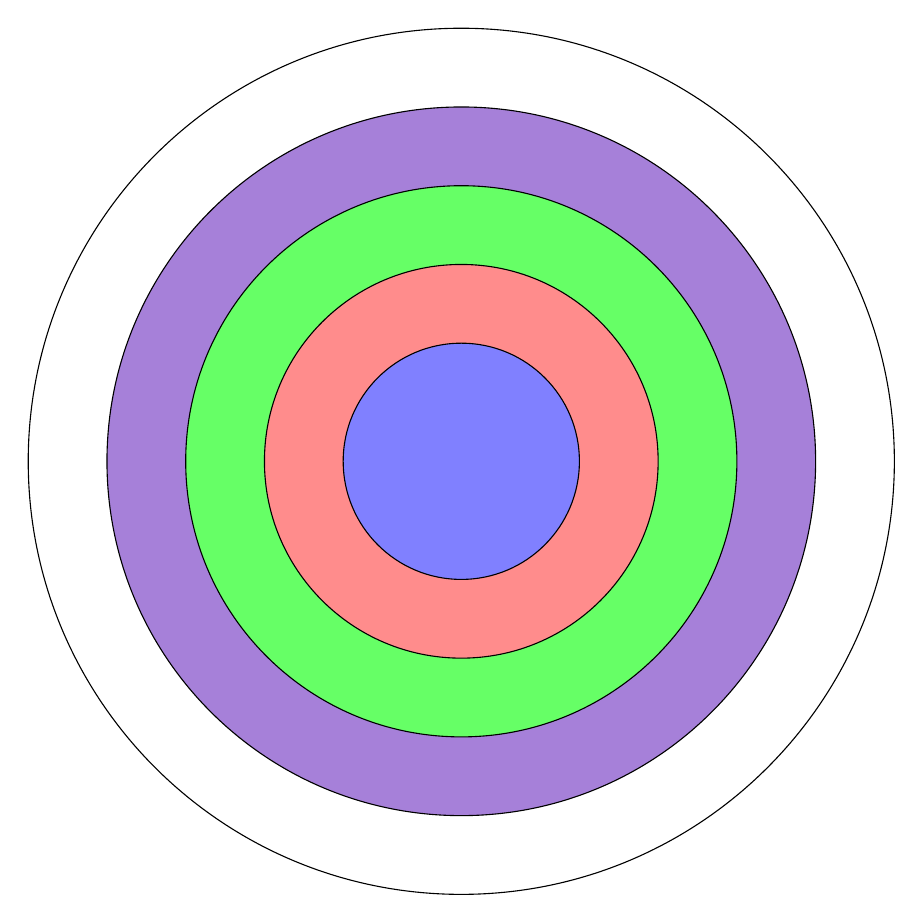
\begin{tikzpicture}
\coordinate (O) at (0,0);

\draw (O) circle (5.5);
\draw[fill=blue!70!red!50!white] (O) circle (4.5);
\draw[fill=green!60] (O) circle (3.5);
\draw[fill=red!45] (O) circle (2.5);
\draw[fill=blue!50] (O) circle (1.5);
\end{tikzpicture}
\end{center}
\fi

\begin{ques}
How do we deal with $\sqrt{-1}$?
\end{ques}

\begin{definition}
The \emph{imaginary constant} is defined to be $i=\sqrt{-1}$
\end{definition}

\begin{note}
This will now allow us to deal with square roots with negative values. If $n>0$, then
\[
\sqrt{-n}=\blank{=\sqrt{-1\cdot n}=\sqrt{-1}\sqrt{n}=i\sqrt{n}}{=\sqrt{-1\cdot n}=\sqrt{-1}\sqrt{n}=i\sqrt{n}}
\]
\end{note}
\begin{exercise}
Simplify $\sqrt{-75}$.
\end{exercise}
\begin{solution}[2in]

\end{solution}
\vspace{0.5em}

\begin{note}
We can simplify powers of $i$ as follows:
\begin{align*}
i&=i\\
i^2&=\blank{(\sqrt{-1})^2=-1}{===========}\\
i^3&=\blank{(i^2\cdot i=-i}{===========}\\
i^4&=\blank{i^2\cdot i^2=(-1)(-1)=1}{===========}\\
i^5&=\blank{i^4\cdot i=1\cdot i=i}{===========}\\
i^6&=\blank{-1}{===========}\\
i^7&=\blank{-i}{===========}\\
&\vdots
\end{align*}
\ifprintanswers This pattern repeats forever.\fi
\end{note}

\begin{exercise}
Simplify $i^{62}$
\end{exercise}
\begin{solution}[2in]

\end{solution}
\vspace{0.5em}

\begin{exercise}
Simplify $i^{19}$
\end{exercise}
\begin{solution}[2in]

\end{solution}
\vspace{0.5em}

\begin{note}
We can also continue the pattern in reverse to get negative powers of $i$:
\begin{align*}
i^0&=\blank{1}{===========}\\
i^{-1}&=\blank{-i}{===========}\\
i^{-2}&=\blank{-1}{===========}\\
i^{-3}&=\blank{i}{===========}\\
&\vdots
\end{align*}
\end{note}

\begin{definition}\label{def: Complex number}
The \emph{complex numbers} (denoted by $\mathbb{C}$) is the set of all
numbers of the form $a+bi$ where $a$ and $b$ are real numbers and $i$
is the imaginary constant.

We call $a+bi$ the standard form of a complex number, calling $a$ the real part
and $b$ the imaginary part.
\end{definition}

\subsection{Addition \& Subtraction}

\begin{exercise}
Compute the following:
\[
(3+2i)+(4-7i)
\]
\end{exercise}
\begin{solution}[1.5in]

\end{solution}
\vspace{0.5em}

\begin{exercise}
Compute the following:
\[
(5+7i)-(-3+2i)
\]
\end{exercise}
\begin{solution}[1.5in]

\end{solution}
\vspace{0.5em}

\subsection{Multiplication}

\begin{exercise}
Compute the following:
\[
3(7-5i)
\]
\end{exercise}
\begin{solution}[2in]

\end{solution}
\vspace{0.5em}

\begin{exercise}
Compute the following:
\[
7i(2+4i)
\]
\end{exercise}
\begin{solution}[2in]

\end{solution}
\vspace{0.5em}

\begin{exercise}
Compute the following:
\[
(-3+7i)(2+5i)
\]
\end{exercise}
\begin{solution}[2in]

\end{solution}
\vspace{0.5em}

\begin{exercise}
Compute the following:
\[
(3+2i)(3-2i)
\]
\end{exercise}
\begin{solution}[3in]

\end{solution}
\vspace{0.5em}

\begin{definition}\label{def: complex conjugates}
The two complex numbers $a+bi$ and $a-bi$ are called \emph{complex conjugates}.
Their product is always $a^2+b^2$ which is real.
\end{definition}

\subsection{Division}

In order to divide complex numbers we will need to use the complex conjugate of
the complex number we are dividing by (the denominator).

\begin{example}
Give the complex conjugates for the following complex numbers:
\begin{itemize}
    \item $5-2i\longleftrightarrow\blank{5+2i}{=====}$
    \vspace{0.5em}
    \item $7+11i\longleftrightarrow\blank{7-11i}{=====}$
    \vspace{0.5em}
    \item $-4-2i\longleftrightarrow\blank{-4+2i}{=====}$
\end{itemize}
\end{example}

\vspace{0.5em}

\begin{exercise}
Divide the following and write your answer in standard form.
\[
\frac{16+22i}{3+i}
\]
\end{exercise}
\begin{solution}[2in]

\end{solution}
\vspace{0.5em}

\newpage

\begin{exercise}
Divide the following and write your answer in standard form.
\[
(17+5i)\div(-2+i)
\]
\end{exercise}
\begin{solution}[3.5in]

\end{solution}
\vspace{0.5em}

\section{Solving Quadratic Equations}

\subsection{Solving by Factoring}

\begin{fact}[The Zero Product Rule]
If $AB=0$, then \blank{$A=0$ or $B=0$}{=========}
\end{fact}

\begin{exercise}
Solve the following for $x$:
\[
x^2+4x-21=0
\]
\end{exercise}
\begin{solution}[2in]

\end{solution}
\vspace{0.5em}

\newpage

\begin{exercise}
Solve the following for $y$:
\[
y^2+8y+12=0
\]
\end{exercise}
\begin{solution}[3.5in]

\end{solution}
\vspace{0.5em}

\begin{exercise}
Solve the following for $x$:
\[
9x^2-26x-3=0
\]
\end{exercise}
\begin{solution}[3.5in]

\end{solution}
\vspace{0.5em}

\subsubsection{The Square Root Property}

\begin{exercise}
Solve $x^2=36$ for $x$.
\end{exercise}
\begin{solution}[1.5in]

\end{solution}

\begin{exercise}
Solve $x^2=81$ for $x$.
\end{exercise}
\begin{solution}[1.5in]

\end{solution}

\subsection{Completing the Square}

This will be using the square root property from above and perfect square trinomials
(see Definition \ref{def: perfect square binomials}). We will change our quadratics as
perfect square trinomials, so that we can take a square root to simplify the problem.

\begin{exercise}
If $x^2+4x-45=0$, solve for $x$.
\end{exercise}
\begin{solution}[2in]

\end{solution}
\vspace{0.5em}

\newpage

\begin{exercise}
If $x^2-12x+11=0$, solve for $x$.
\end{exercise}
\begin{solution}[2in]

\end{solution}
\vspace{0.5em}

\subsection{The Quadratic Formula}

Now completing the square works to solve any quadratic equation, but what if we
tried to complete the square on the general quadratic?

\begin{example}
If $ax^2+bx+c=0$, solve for $x$.
\end{example}
\begin{solution}[3in]

\end{solution}

\newpage

\begin{prop}[The Quadratic Formula]\label{prop: Quadratic Formula}
If $ax^2+bx+c=0$, then
\[
x=\ifprintanswers\frac{-b\pm\sqrt{b^2-4ac}}{2a}\else\phantom{\frac{-b\pm\sqrt{b^2-4ac}}{2a}}\fi
\]
\end{prop}
\vspace{0.5em}

\begin{definition}\label{def: discriminant}
For a quadratic equation $ax^2+bx+c=0$, the \emph{discriminant} is
$b^2-4ac$, and it tells us about the types of
solutions to said equation.

There are 3 (really 4) cases:
\begin{itemize}
    \item $b^2-4ac<0\Rightarrow$ \blank{2 complex solutions}{2 complex solutions}
    \item $b^2-4ac=0\Rightarrow$ \blank{1 rational solution}{1 rational solution}
    \item $b^2-4ac>0$ and
    \begin{itemize}
        \item it IS a perfect square $\Rightarrow$ \blank{2 (distinct) rational solutions}{2 (distinct rational solutions}
        \item it IS NOT a perfect square $\Rightarrow$ \blank{2 irrational solutions}{2 irrational solutions}
    \end{itemize}
\end{itemize}
\end{definition}
\vspace{0.5em}

\begin{exercise}
Find the discriminant and solve $-4x^2+5x+3=0$.
\end{exercise}
\begin{solution}[3in]

\end{solution}
\vspace{0.5em}

\newpage

\begin{exercise}
Find the discriminant and solve $4n^2-20n+25=0$.
\end{exercise}
\begin{solution}[3in]

\end{solution}
\vspace{0.5em}

\section{More Equations and Some Applications}
\subsection{Using the Greatest Common Factor}

\begin{exercise}
Solve $4x^4=16x^2$
\end{exercise}
\begin{solution}[2in]

\end{solution}
\vspace{0.5em}

\begin{exercise}
Solve $9x^4=81x^2$
\end{exercise}
\begin{solution}[1.5in]

\end{solution}
\vspace{0.5em}

\subsection{Factoring by Grouping}
\begin{exercise}
Solve $x^3-5x^2-4x+20=0$.
\end{exercise}
\begin{solution}[2.2in]

\end{solution}
\vspace{0.5em}

\begin{exercise}
Solve $x^3-8x^2-9x+72=0$.
\end{exercise}
\begin{solution}[2.2in]

\end{solution}
\vspace{0.5em}

\begin{exercise}
Solve $x^3+7x^2-x-7=0$.
\end{exercise}
\begin{solution}[2.2in]

\end{solution}
\vspace{0.5em}

\newpage
\subsection{Polynomials in Quadratic Form}

\begin{exercise}
Solve $(x-5)^2+(x-5)-2=0$.
\end{exercise}
\begin{solution}[4in]

\end{solution}
\vspace{0.5em}

\begin{exercise}
Solve $(x-7)^2-7(x-7)+10=0$.
\end{exercise}
\begin{solution}[3in]

\end{solution}
\vspace{0.5em}

\newpage
\subsection{Absolute Value Equations}
\begin{definition}\label{def: absolute value}
The \emph{absolute value} of a number $n$, written $\vert n\vert$, is the
distance from $n$ to $0$ on the number line (i.e. it is the positive version of $n$).
\end{definition}

\begin{example}
If $\vert x\vert=5$, then either $x=5$ or $x=-5$
\end{example}

This means that absolute value equations are just two problems in one. A positive equation and a negative equation.

\begin{exercise}
If $\vert-12x-7\vert-8=2$, solve for $x$.
\end{exercise}
\begin{solution}[3.5in]

\end{solution}
\vspace{0.5em}

\begin{exercise}
Solve $2\vert x+1\vert+7=10$ for $x$.
\end{exercise}
\begin{solution}[3in]

\end{solution}
\vspace{0.5em}

\begin{exercise}
Solve the following for $x$:
\[
\vert 3x-5\vert-11=-9
\]
\end{exercise}
\begin{solution}[3in]

\end{solution}
\vspace{0.5em}

\subsection{Radical Equations}

Our goal will be to get rid of the radical in the problem.

\begin{exercise}
Solve the following for $x$:
\[
\sqrt{8x-23}+2=x
\]
\end{exercise}
\begin{solution}[4in]

\end{solution}

\begin{exercise}
Solve:
\[
\sqrt{-2x+8}=x
\]
\end{exercise}
\begin{solution}[3in]

\end{solution}
\vspace{0.5em}

\begin{exercise}
Solve:
\[
\sqrt{-x+4}+\sqrt{5x+1}=3
\]
\end{exercise}
\begin{solution}[4in]

\end{solution}

\newpage

\begin{exercise}
Solve:
\[
\sqrt{-2x+2}+\sqrt{x+2}=-3
\]
\end{exercise}
\begin{solution}[2in]

\end{solution}
\vspace{0.5em}

\subsection{Rational Exponent Equations}

Recall that the square root is the same as the \blank{$1/2$}{1/2} power, so
in general we take
\[
\Big(\big(~~\big)^{m/n}\Big)^{\blank{n}{n}/\blank{m}{m}}
\]

\begin{exercise}
Solve $x^{7/6}=128$ for $x$.
\end{exercise}
\begin{solution}[2in]

\end{solution}
\vspace{0.5em}

\begin{exercise}
Find $x$ when $\dl x^{-3/2}=\frac{1}{125}$
\end{exercise}
\begin{solution}[2in]

\end{solution}
\vspace{0.5em}

\begin{exercise}
Solve for $x$ when $\dl (x-1)^{-4/3}=\frac{1}{81}$
\end{exercise}
\begin{solution}[3.5in]

\end{solution}
\vspace{0.5em}

\begin{exercise}
Solve the following for $x$:
\[
7x^4-189x^{13/4}=0
\]
\end{exercise}
\begin{solution}[4in]

\end{solution}
\vspace{0.5em}
\begin{exercise}
Solve the following for $x$:
\[
4x^3-36x^{7/3}=0
\]
\end{exercise}
\begin{solution}[2in]

\end{solution}
\vspace{0.5em}

\subsection{More Rational Equations}

\begin{note}
We still need to check what makes our denominators equal to 0
\end{note}
\vspace{0.5em}

\begin{exercise}
If $\dl \frac{6x+5}{x+2}-\frac{1}{x}=-\frac{2}{x^2+2x}$, find $x$.
\end{exercise}
\begin{solution}[4in]

\end{solution}
\vspace{0.5em}

\newpage

\section{Linear, Compound, and Absolute Value Inequalities}\label{sec: linear and absolute inequalities}

We need a shared language to discuss these problems because
the answers are not just single numbers they are sets (or
collections) of numbers like the following:

\begin{example}\label{example: numberline}
The set of all real numbers greater than or equal to 1.

\vspace{0.1in}

\begin{center}
\begin{tikzpicture}
\node(N)                        {$-\infty$};
\node(P)    [right=8cm of N]    {$\infty$};

\draw[>=stealth,black,<->] (N) -- (P);
\end{tikzpicture}
\end{center}
\end{example}

\subsection{Interval Notation}

\[
\begin{tabular}{c|c}
Set Builder Notation & Interval Notation \\
\hline
& \\
$\{x\mid a<x<b\}$ & \blank{$(a,b)$}{$(a,b)$}\\
& \\
$\{x\mid a\le x\le b\}$ & \blank{$[a,b]$}{$[a,b]$} \\
& \\
$\{x\mid a<x\le b\}$ & \blank{$(a,b]$}{$(a,b]$} \\
& \\
$\{x\mid a\le x<b\}$ & \blank{$[a,b)$}{$[a,b)$} \\
& \\
$\{x\mid a\le x\}$ & \blank{$[a,\infty)$}{$[a,\infty)$} \\
& \\
$\{x\mid x<b\}$ & \blank{$(-\infty,b)$}{$(-\infty,b)$} \\
\end{tabular}
\]

\begin{exercise}
Write the number line from Example \ref{example: numberline} in
interval notation.
\end{exercise}
\begin{solution}[1in]

\end{solution}
\vspace{0.5em}

\begin{definition}
\text{}
\begin{itemize}
    \item \blank{$\cup$}{$\cup$} -- denotes the \emph{union} which means ``or''.
    \item \blank{$\cap$}{$\cap$} -- denotes the \emph{intersection} which means ``and''.
\end{itemize}
\end{definition}

\newpage

\begin{exercise}
Use interval notation to express the following:

The set of all real numbers greater than $-1$ and less than $0$.
\end{exercise}
\begin{solution}[2in]

\end{solution}
\vspace{0.5em}

\begin{exercise}
Use interval notation to express the following:

The set of all real numbers greater than $-7$ and less than or equal
to $5$.
\end{exercise}
\begin{solution}[2in]

\end{solution}
\vspace{0.5em}

\begin{exercise}
Use interval notation to express the following:

The set of all real numbers greater than or equal to $4$
or less than $2$.
\end{exercise}
\begin{solution}[2in]

\end{solution}
\vspace{0.5em}

\newpage

\subsection{Properties of Inequalities}

\subsubsection*{Addition Property}
If $a<b$, then for a real number $c$ \blank{$a+c<b+c$}{$a+c<b+c$}.

\subsubsection*{Multiplication Property}
\begin{itemize}
    \item If $a<b$ and $c>0$, then \blank{$ac<bc$}{$ac<bc$}.
    \item If $a<b$ and $c<0$, then \blank{$ac>bc$}{$ac>bc$}.
\end{itemize}

\begin{exercise}
If $x+10\leq4$, solve for $x$.
\end{exercise}
\begin{solution}[1in]

\end{solution}
\vspace{0.5em}

\begin{exercise}
Find $x$ when $-5x-2\leq8$.
\end{exercise}
\begin{solution}[2in]

\end{solution}
\vspace{0.5em}

\begin{exercise}
Solve $-16x+8\geq-9x-13$ for $x$.
\end{exercise}
\begin{solution}[2in]

\end{solution}
\vspace{0.5em}

\newpage

\begin{exercise}
Find $x$ when $-10x+12>-8x-10$.
\end{exercise}
\begin{solution}[2in]

\end{solution}
\vspace{0.5em}

\subsection{Compound Inequalities}

\begin{exercise}
Solve $2x-3\leq4x+3<2x+5$ for $x$.
\end{exercise}
\begin{solution}[2in]

\end{solution}
\vspace{0.5em}

\begin{exercise}
Find $x$ if $-4x-10<-2x-8\leq-4x+10$.
\end{exercise}
\begin{solution}[2in]

\end{solution}
\vspace{0.5em}

\newpage

\subsection{Absolute Value Inequalities}

Recall that absolute values turn one problem into two!

\begin{exercise}
Solve $\vert x-6\vert+2=4$ for $x$.
\end{exercise}
\begin{solution}[2in]

\end{solution}
\vspace{0.5em}

With inequalities we either have an ``and'' or an ``or'' problem.

\begin{note}
Here is a trick to remember:
\begin{itemize}
    \item And -- \blank{Less Th\underline{an}}{Less Th\underline{an}} 
    \item Or -- \blank{Great``or''}{Great``or''}
\end{itemize}
\end{note}

\begin{exercise}
Solve $\vert2x+6\vert<18$ for $x$.
\end{exercise}
\begin{solution}[2in]

\end{solution}
\vspace{0.5em}

\newpage

\begin{exercise}
Solve $-7\vert x+12\vert\leq-14$ for $x$.
\end{exercise}
\begin{solution}[2in]

\end{solution}
\vspace{0.5em}

\begin{exercise}
Solve $2\vert x-12\vert+1\leq23$ for $x$.
\end{exercise}
\begin{solution}[2in]

\end{solution}

\begin{exercise}
Solve $\vert x-5\vert\leq-2$ for $x$.
\end{exercise}
\begin{solution}[2in]

\end{solution}
\vspace{0.5em}